\chapter{Conclusions and Future Work}
\label{sec:ch7}

The work shown throughout this document can also be found in Refs. \cite{cris1,cris2, cris3}. This section reports on the conclusions and future work stemming from this thesis.

\section{Conclusions}

\subsection{RDTs and Resonance Compensation in the Recycler Ring}

The measurement and subsequent cancellation of RDTs was investigated in depth in Ch. \ref{sec:ch4}. It was shown that third order RDTs in the Recycler Ring can be measured and, afterwards, cancelled with the compensation sextupoles in place. Furthermore, optimization procedures have been developed in order to have this compensation with physics-informed input and/or with numerical optimization. The Recycler Ring now has a resonance compensation method for when large tune spreads are present. Depending on the operational tunes, any setting in the compensation sextupoles from Fig. \ref{fig:lossmaps} can be enabled to cope with space-charge-induced losses. This is a new operational feature that can be enabled on demand and will be specially useful for the PIP-II era. 

\subsection{Physics-Informed vs. Optimization-Based Compensation}

Chapters \ref{sec:ch4} and \ref{sec:ch5} showed two different approaches to the same problem of resonance compensation. The first one performed at the Fermilab Recycler Ring showed how to implement the response matrix approach, which can be traced to some underlying physics principles. On the other hand, Ch. \ref{sec:ch5} shows how to implement numerical optimization algorithms for compensating multiple resonance lines at the CERN PS Booster. Nevertheless, this last approach had no direct physics input. The distinction between a physics-informed approach and a numerical-optimization approach summarizes the differences between both chapters. The numerical-optimization approach is a brute-force one that can be carried out without no physics input---just by minimizing the losses in the resonance lines with the compensation sextupoles. Nevertheless, the physics-informed compensation can significantly enhance the numerical optimization by constraining a window in parameter space where the solution lies. The best approach to resonance compensation is to use a hybrid scheme where the response matrix method sets the limits in parameter space for a subsequent and faster numerical optimization. 

\subsection{High-Intensity Resonance Compensation}

For current operations of the Fermilab Accelerator Complex, the third-order resonance compensation scheme developed in this work will not have an effect on reducing losses in the Recycler Ring. The current tune spreads in the RR are not large enough for the third order resonances to be specially harmful to operations. The beam coming out of Booster grows exponentially with the beam intensity, as it was shown in Fig. \ref{fig:tunespread}. Thus, saturating the tune spread at values close to 0.02---not particularly large. The losses in the Recycler Ring are purely emittance-dominated for current operations. They are not related to space charge effects. Nonetheless, the resonance compensation scheme still is beneficial to operations at high intensities when close to the third-order resonances. The operational tune should still keep as far as possible from these lines.  

\subsection{Transverse Dampers and High-Intensity Compensation}

Section \ref{sec:ch6dampers} showed how the transverse dampers have an effect on the resonance compensation scheme. Figure \ref{fig:dampers7} reinforces this statement by showing the beam survival ratio at a high intensity of 4.5e10 ppb without compensation and dampers on (bare machine), with compensation and dampers on, and with compensation and dampers off. Ultimately, the dampers degrade the quality of the compensation. In particular, when turned off, the overall beam survival ratio increases. The configuration of the dampers---gain and phase of feedback---has been optimized away from the resonance lines. When the tunes are set close to the third order resonance lines, the dampers settings will create beam size growth. They are not optimized to run in this region, and will cause harmful effects on the beam, even with the resonance compensation scheme enabled.

\begin{figure}[H]
    \centering
    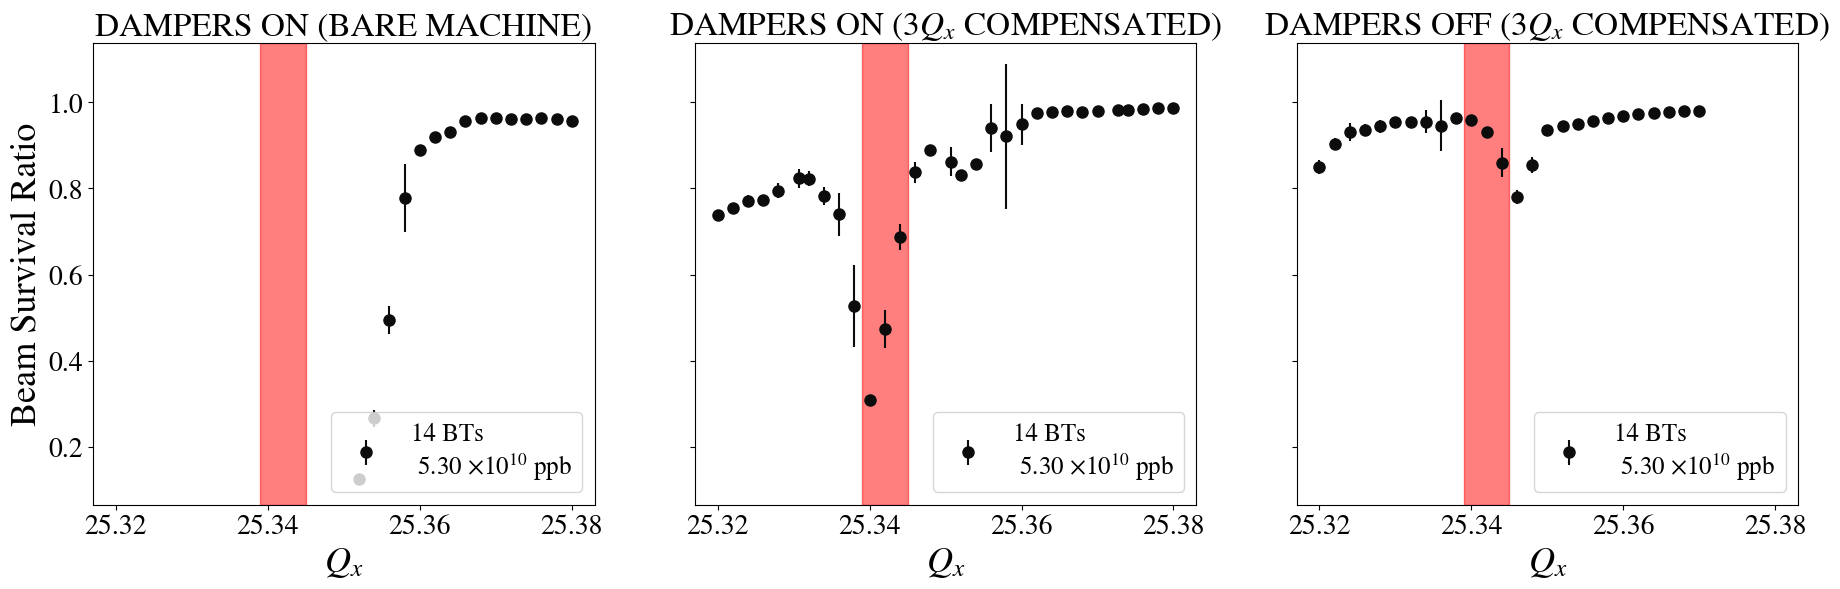
\includegraphics[width=\columnwidth]{chapter7/dampers_config.png}
    \caption{Transverse damper effect on resonance compensation for bare machine + dampers ON, $3Q_x$ compensated + dampers ON, and $3Q_x$ compensated + dampers OFF configuration. The red band corresponds to the $3Q_x$ stop band at an intensity of 0.5 ppb with dampers ON.}
    \label{fig:dampers7}
\end{figure}

\section{Future Work}

\subsection{Verification of Newly-Installed Sextupoles}

Section \ref{sec:compensate} explained the motivation behind installing additional sextupoles that would bring down the currents needed to compensate $3Q_x=76$ and $Q_x+ 2Q_y = 74$. Subsequently, Sec. \ref{sec:addsexts} explained the procedure used in order to pin down the new locations for two new compensation sextupoles. These sextupoles have been installed in the Recycler. There is still future work to be done regarding the commissioning and connection of the new 620 sextupoles. The sextupoles and their power supplies need to be interfaced with ACNET. Furthermore, the resonance compensation enhancement still needs to verified by means of performing an RDT scan. Specifically, the response matrix coefficients corresponding to these new sextupoles need to be measured and calculated. All of this, following the procedure outlined in Secs. \ref{sec:rdtmeasure} and \ref{sec:compensate}. Figure \ref{fig:new620sexts} shows a picture of the newly installed sextupoles.

\begin{figure}[H]
    \centering
    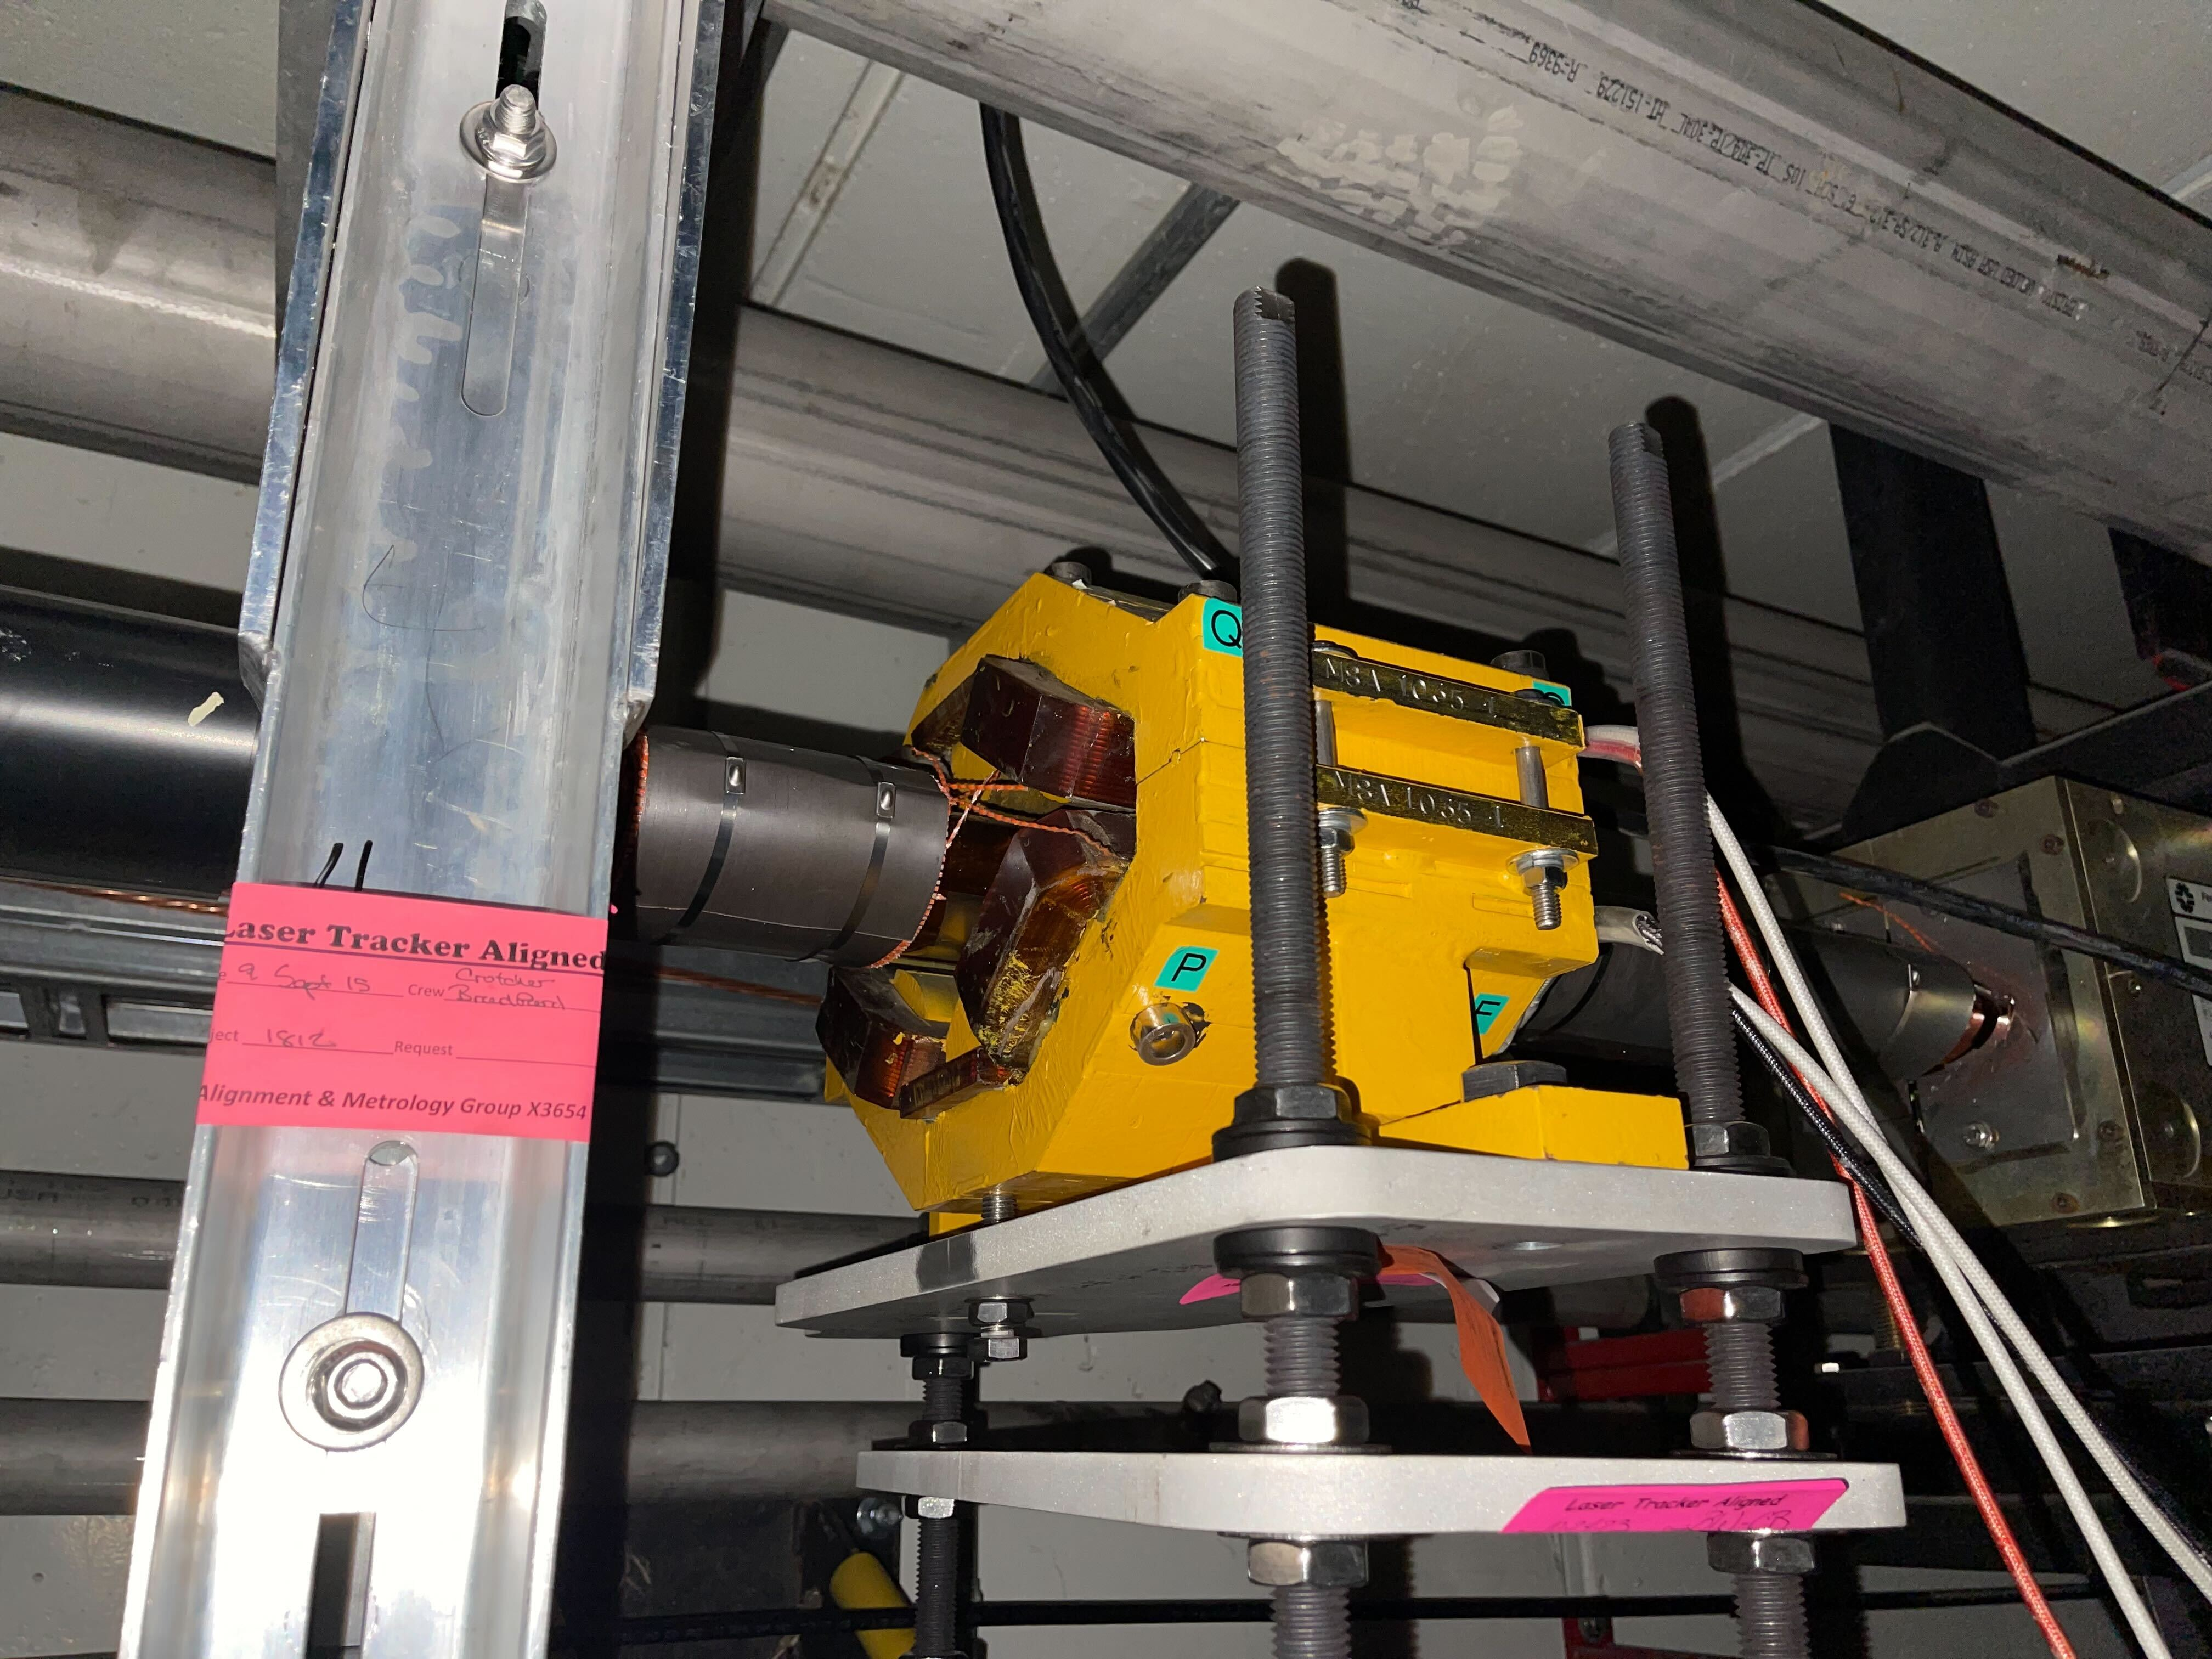
\includegraphics[width=\columnwidth]{chapter7/620_sext.jpg}
    \caption{Newly installed compensation sextupoles in the 620 section.}
    \label{fig:new620sexts}
\end{figure}

\subsection{Resonances and Transverse Dampers at High Intensities}

It was shown in Sec. \ref{sec:ch6dampers} that the transverse dampers in the Recycler Ring can interact with betatron resonance lines depending on their configuration. It would be interesting to perform experiments with the configuration of these dampers in order to fully characterize these effects, i.e., change the gain and phase of the dampers and study their effect on the strength of the resonance lines. Furthermore, it would also be interesting to use the dampers as anti-dampers in order to sustain betatron oscillations. With this configuration, one could perform tune measurements, and perhaps evaluate this alternative method to measure RDTs. This would be similar to having an AC dipole installed in the Recycler.  

\subsection{Effect of MI Ramp on RDTs}

The ultimate objective of this work is to have this resonance compensation scheme fully characterized in order to incorporate it into high intensity operations. Nevertheless, there is one additional factor that has been identified to also play a role in this effort. This one stems from the fact that the Main Injector and the Recycler Ring share the same tunnel. It has been shown that the MI acceleration ramp changes the beam dynamics inside the RR. In particular, it introduces orbit distortions and tune shifts depending on the position of the ramp \cite{mionrr}. There is an ongoing effort in order to characterize any higher order magnetic effect from the MI to RR, e.g., any sextupole term that is being introduced by the MI acceleration ramp. The first results have shown that the compensation currents change depending on the location of the study event with respect to the MI acceleration ramp. Therefore, in the future, the resonance compensation described hereinabove should be modified to accommodate this effect to be fully operational.

\subsection{Limits of Resonance Compensation}

Chapter \ref{sec:ch4}, specifically Sec. \ref{sec:lossmaps}, shows how individual and different pairs of resonance lines can be compensated in the Recycler Ring. Nevertheless, there is still a question if all the four third-order resonance lines can be compensated simultaneously. While the previous thesis does not explicitly answer this question, it does contribute to a better understanding of the resonance lines. The source of these third-order resonance lines is a systematic third order term in the permanent combined function magnets distributed around the ring. The fact that these are systematic does not allow for a straight-forward compensation of the four resonance lines. Every time a larger number of resonance lines are trying to be corrected, the currents in the compensation sextupoles increase. Therefore, one would need more compensation sextupoles around the ring at specific locations to bring down these currents, just at it was done in Sec. \ref{sec:addsexts}. Ultimately, the approach to follow would be to try to minimize the RDT fluctuations around the ring with the least amount of correctors. Such is the approach in Ref. \cite{rdtfluct}. Another thing to take into account for future theoretical studies, is that introducing too much sextupole in the ring might take the machine closer to an anharmonic regime. In this anharmonic regime the resonances will not be necessarily straight lines, but rather polynomial curves as a result of motion in a 4D coupled phase space \cite{fixedlines1,fixedlines2}.  These are considerations for future exploration on the limits of resonance compensation driven by systematic terms around the ring.  

\subsection{Space Charge RDTs}

Equation \ref{eq:hfinal} shows how the lattice elements and the space charge potential drive betatron resonances. It would be interesting to explore further how to measure space charge resonance driving terms (SCRDTs) and their effect on the operation of the Recycler Ring. Without taking into account any collective instabilities, the ultimate limit of the Recycler Ring will be dictated by how strong these third order lines become in the space-charge dominated regime. The current future of the Main Injector and Recycler Ring lies in high-intensity beam. As the space charge potential grows for the Fermilab beams, it is important to quantify all effects from high intensity operation---being SCRDTs one of them.
